\section{Sơ đồ RTL và FSM}

\subsection{Sơ đồ khối RTL}
\begin{figure}[H]
    \centering
    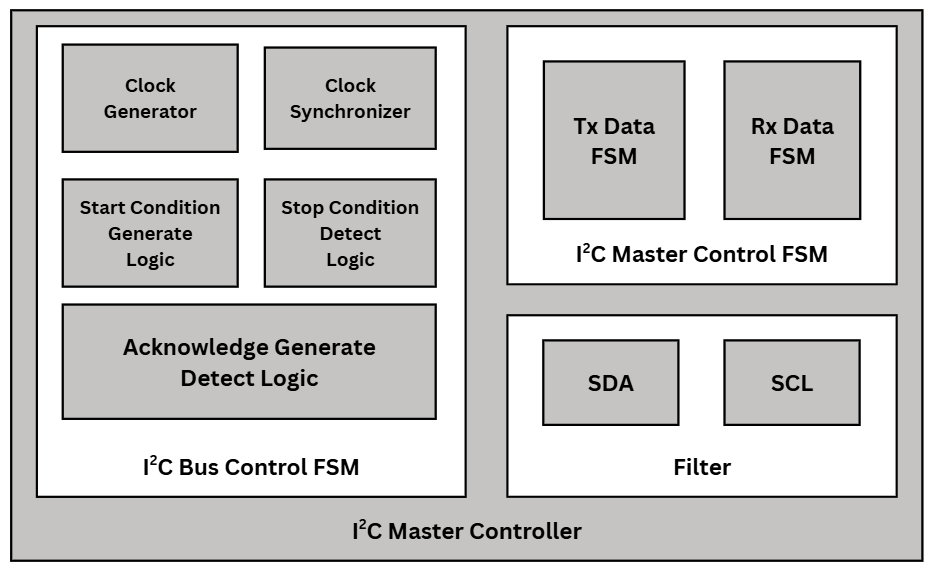
\includegraphics[width=0.92\textwidth,keepaspectratio]{figures/i2c_from_docx/functional_block_diagram.png}
    \caption{Sơ đồ khối chức năng RTL (Clock Gen, START/STOP, ACK, Tx/Rx FSM, SCL/SDA)}
    \label{fig:rtl}
\end{figure}

Theo Hình \ref{fig:rtl}, lõi I\textsuperscript{2}C được phân rã thành:
\begin{itemize}[leftmargin=1.2cm]
    \item \textbf{I\textsuperscript{2}C Bus Control FSM}: gồm \emph{Clock Generator}, \emph{Clock Synchronizer}, logic tạo/phát hiện START/STOP, và khối \emph{Acknowledge Generate/Detect Logic}. Đây là phần quyết định timing bit trên SDA/SCL và xử lý ACK/NACK.
    \item \textbf{I\textsuperscript{2}C Master Control FSM}: chứa \emph{Tx Data FSM} và \emph{Rx Data FSM}, phối hợp để dịch bit trong 1 byte và handshake dữ liệu với CPU.
    \item \textbf{Filter}: tách lọc đường \textbf{SDA} và \textbf{SCL} để nhận/điều khiển pad.
\end{itemize}

\subsection{I2C Bus Control FSM}
\begin{figure}[H]
    \centering
    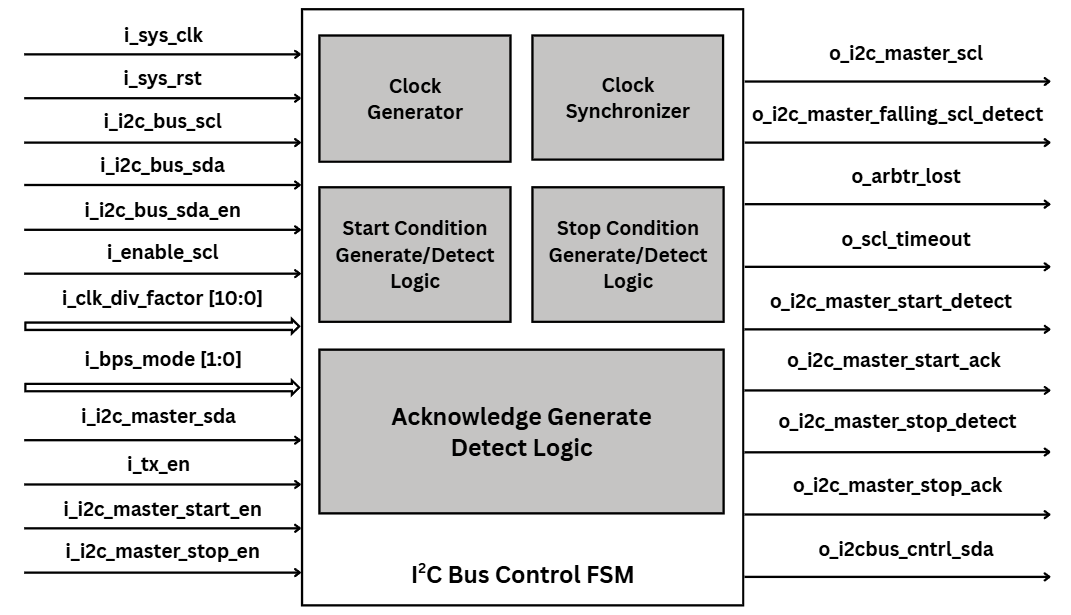
\includegraphics[width=0.88\textwidth,keepaspectratio]{figures/i2c_from_docx/i2c_bus_control_fsm.png}
    \caption{I2C Bus Control FSM}
    \label{fig:bus_fsm}
\end{figure}

Hình \ref{fig:bus_fsm} cho thấy Bus FSM nhận các tín hiệu bus (\texttt{i\_i2c\_bus\_scl}, \texttt{i\_i2c\_bus\_sda}) và điều khiển các tín hiệu tạo START/STOP (\texttt{i\_i2c\_master\_start\_en}, \texttt{i\_i2c\_master\_stop\_en}) cùng enable kéo SDA (\texttt{i\_i2c\_bus\_sda\_en}, \texttt{i\_tx\_en}). Khối này xuất:
\begin{itemize}[leftmargin=1.2cm]
    \item SCL điều khiển bởi master (\texttt{o\_i2c\_master\_scl}) và các cờ timing như \texttt{o\_i2c\_master\_falling\_scl\_detect}.
    \item Cờ trạng thái/ngoại lệ bus: \texttt{o\_arbtr\_lost} (mất arbitration), \texttt{o\_scl\_timeout}.
    \item Các cờ nhận diện/ack: \texttt{o\_i2c\_master\_start\_detect}, \texttt{o\_i2c\_master\_start\_ack}, \texttt{o\_i2c\_master\_stop\_detect}, \texttt{o\_i2c\_master\_stop\_ack}.
    \item Điều khiển SDA mức bus: \texttt{o\_i2cbus\_cntrl\_sda}.
\end{itemize}

\subsection{I2C Master Control FSM}
\begin{figure}[H]
    \centering
    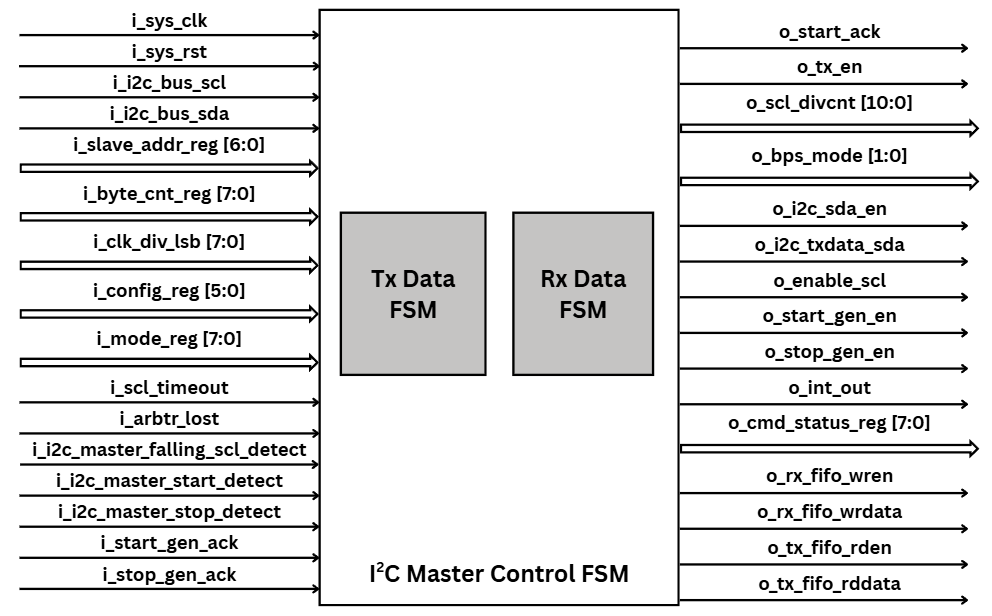
\includegraphics[width=0.88\textwidth,keepaspectratio]{figures/i2c_from_docx/i2c_master_control_fsm.png}
    \caption{I2C Master Control FSM}
    \label{fig:master_fsm}
\end{figure}

Hình \ref{fig:master_fsm} mô tả các interface của Master FSM. Phía vào gồm \texttt{i\_slave\_addr\_reg[6:0]}, \texttt{i\_byte\_cnt\_reg[7:0]}, \texttt{i\_clk\_div\_lsb[7:0]}, \texttt{i\_config\_reg[5:0]}, \texttt{i\_mode\_reg[7:0]} và các cờ phản hồi từ Bus FSM như \texttt{i\_i2c\_master\_start\_detect}, \texttt{i\_i2c\_master\_stop\_detect}, \texttt{i\_i2c\_master\_falling\_scl\_detect}, \texttt{i\_arbtr\_lost}, \texttt{i\_scl\_timeout}.

Phía ra gồm:
\begin{itemize}[leftmargin=1.2cm]
    \item Enable/tín hiệu điều khiển bus: \texttt{o\_tx\_en}, \texttt{o\_enable\_scl}, \texttt{o\_i2c\_sda\_en}, \texttt{o\_start\_gen\_en}, \texttt{o\_stop\_gen\_en}.
    \item Đường dữ liệu SDA TX: \texttt{o\_i2c\_txdata\_sda}.
    \item Tham số timing: \texttt{o\_scl\_divcnt[10:0]} và mode \texttt{o\_bps\_mode[1:0]}.
    \item Giao tiếp FIFO/CPU: \texttt{o\_rx\_fifo\_wren}, \texttt{o\_rx\_fifo\_wrdata}, \texttt{o\_tx\_fifo\_rden}, \texttt{o\_tx\_fifo\_rddata}, và trạng thái \texttt{o\_cmd\_status\_reg[7:0]}.
    \item Ngắt/ack: \texttt{o\_int\_out}, \texttt{o\_start\_ack}.
\end{itemize}

